\documentclass[t, 10pt]{beamer}
%%\documentclass[t,handout]{beamer}

\usepackage{graphicx}
\usepackage{epsfig}
\usepackage{psfrag}
\usepackage[english]{babel}
\usepackage{color}
\usepackage{natbib}

%Mathematics packages
\usepackage{amsmath}
\usepackage{mathrsfs}
\usepackage{amsfonts}
\usepackage{enumerate}

\graphicspath{{./images/}} % Figures path - used in graphicx

\selectcolormodel{cmyk}

\mode<presentation>

%THEMES - Please refer to these chapters in the beamer documentation.
% Presentation themes : Chapter 15
% Color themes : Chapter 17
% Font themes : Chapter 18


\usetheme{Pittsburgh}
\usecolortheme{orchid}
\usefonttheme{default}

\setbeamertemplate{bibliography item}[text]
\setbeamercovered{transparent=7}

%---------------------------Title frame definition------------------------------------- 

\title{Policy Overlay Networks}
\author [Chris]{Christopher C. Lamb}
\institute[University of New Mexico]{
\inst {}Department of Electrical and Computer Engineering\\
University of New Mexico}
\date{June 10, 2011}
\titlegraphic{
\begin{figure} 

\includegraphics[width = 7cm]{UNM}
\end{figure}}

% Delete this, if you do not want the table of contents to pop up at
% the beginning of each subsection:
%\AtBeginSubsection[]
%{
%  \begin{frame}<beamer>
%    \frametitle{Outline}
%     \tableofcontents[currentsection,currentsubsection]
%  \end{frame}
%}

\begin{document}

\begin{frame}
\titlepage
\end{frame}

% This command will make the logo appear on all frames excluding the title frame.
\logo {
\includegraphics[width = 2.5cm]{UNM}}

\begin{frame}
\frametitle{Outline}
\tableofcontents 
\end{frame}

\section{Introduction}
\begin{frame}
\frametitle{Introduction}
Federal computing systems are facing a troubling future.  They are:
\pause
\begin{itemize}
\item \textit{Expensive} --- They do not use current commercial resources and use costly partitioning schemes
\pause
\item \textit{Unreliable} --- Too reliant on outmoded security approaches
\pause
\item \textit{Slow} --- Information is manually reviewed too often leading to the right people being unable to get the right information in time 
\end{itemize}
\
\newline
\newline
\newline
\pause
\textit{They need to be re-imagined to take advantage of radical shifts in computational provisioning.}
\end{frame}
\section{Motivation --- Cloud-centric Usage Management}

% Outline
% I. Frame the problem (use the AF proposal for this)
% II. Outline current solutions from UCDMO using guards
% III. Discuss problems (use pro/con list)
% IV. Frame specific challenges using slides II, III

\begin{frame}
\frametitle{The Problem}
Current policy-centric systems are being forced to move to cloud environments and build much more open systems:
\newline
\newline
\newline
"...It is imperative to  effectively exchange information among components, Federal agencies, coalition partners, foreign governments and international organizations as a critical element of our efforts to defend the nation and execute national strategy..."\cite{proposal:info-sharing-strategy}
\newline
\begin{footnotesize}\textit{--- DoD Information Sharing Strategy}\end{footnotesize}
\newline
\newline
\newline
"...The CIO of the National Security Agency is focusing on IT architecture and a cloud-centric approach to sharing information..."\cite{proposal:nsa-cloud}
\newline
\begin{footnotesize}\textit{--- Informationweek}\end{footnotesize}
\end{frame}

\begin{frame}
\frametitle{The Problem}
Cloud systems may save money, provide more flexibility, but they also \cite{proposal:privacy-security-trust-cloud}:
\begin{itemize}
\item \textit{Are Not Private} ---
\item \textit{Are Less Secure} ---
\item \textit{Cannot Be Trusted} ---
\end{itemize}
\end{frame}
%\section{Closest Related Work}
\begin{frame}
\frametitle{Related Work}
\begin{beamerboxesrounded}[shadow]{}
\textbf{Protecting domains...}
\end{beamerboxesrounded}
\textit{Domains} exist below a specific overlay, and trusted secure paths between domains corresponding to a single overlay network are negotiated \textit{a priori} and then used by the overlay \cite{4457175}
\newline
\newline
\textbf{May be useful in this work, but the authors are a bit obtuse on the application of their ideas}
\newline
\newline
\textit{Using specific policies in a policy layer to protect the underlying network strata from abuse by overlays \cite{foo}}
\newline
\newline
\textbf{Doesn't really address content-centric policies}
\newline
\newline
\begin{beamerboxesrounded}[shadow]{}
\textbf{...not content.}
\end{beamerboxesrounded}
\end{frame}
%\section{System Architecture}
\begin{frame}
\frametitle{System Architecture}
What would this kind of overlay system look like?
\begin{itemize}
\item<2-> \textit{Meta-Model}
\item<3-> \textit{Non-Hierarchical Overlays}
\item<4-> \textit{Hierarchical Overlays}
\item<5-> \textit{Ontologies and Taxonomies}
\end{itemize}
\
\newline
\newline
\pause
\textit{...and what would the migration path to these systems look like?}
\end{frame}

\begin{frame}[t]
\frametitle{System Architecture - Level $\phi$}
\begin{figure}[!t]
\centering
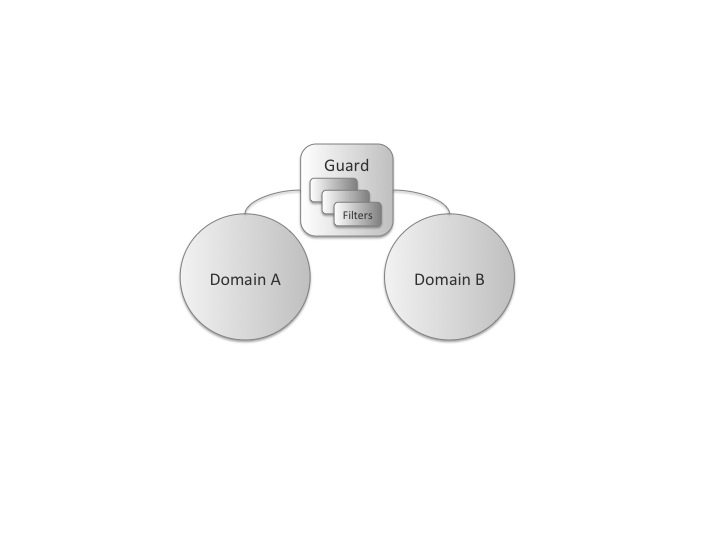
\includegraphics[width=3.4in]{model-phi}
\label{fig:model:phi}
\end{figure}
\end{frame}

\begin{frame}[t]
\frametitle{System Architecture - Level $\alpha$}
\begin{figure}[!t]
\centering
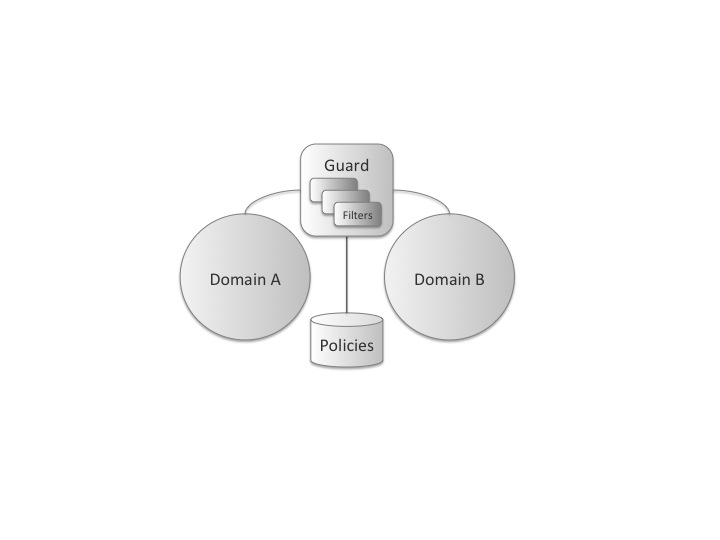
\includegraphics[width=3.4in]{model-alpha}
\label{fig:model:alpha}
\end{figure}
\end{frame}

\begin{frame}[t]
\frametitle{System Architecture - Level $\beta$}
\begin{figure}[!t]
\centering
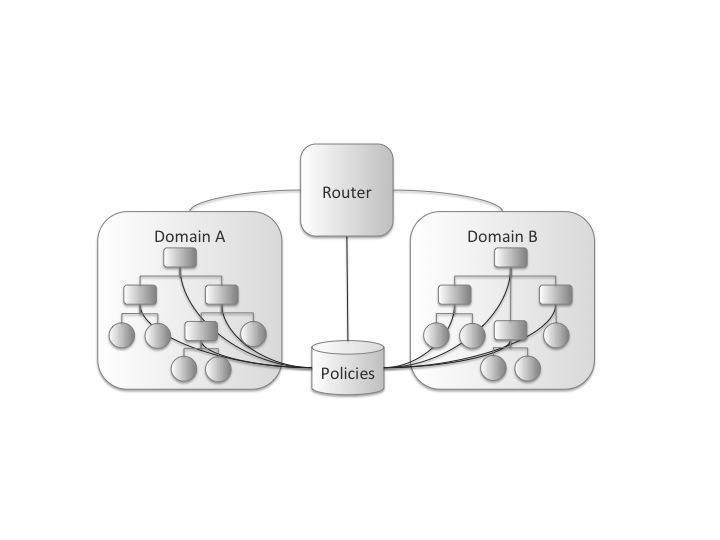
\includegraphics[width=3.4in]{model-beta}
\label{fig:model:beta}
\end{figure}
\end{frame}

\begin{frame}[t]
\frametitle{System Architecture - Level $\gamma$}
\begin{figure}[!t]
\centering
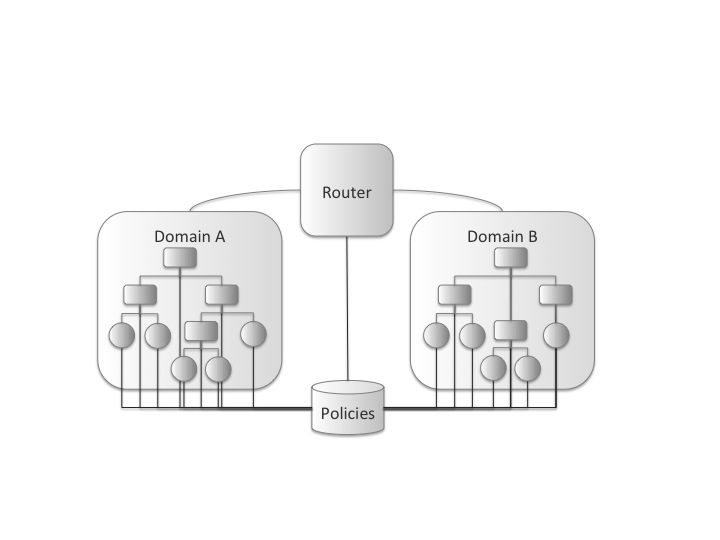
\includegraphics[width=3.4in]{model-gamma}
\label{fig:model:gamma}
\end{figure}
\end{frame}

\begin{frame}[t]
\frametitle{System Architecture - Level $\delta$}
\begin{columns}[t]
\column{.5\textwidth}
Level 3 system 
\column{.5\textwidth}
Fully Integrated Policy Aware Decentralized System
\end{columns}
\end{frame}
%\section{Logical Demonstration}
\begin{frame}
\frametitle{Logical Demonstration}
\end{frame}
%\section{Conclusions}
\begin{frame}
\frametitle{Conclusions}
\begin{beamerboxesrounded}[shadow]{Contribution of Work}
The unique contribution of this work is a quantitative analysis of policy-centric overlay network options, associated taxonomies of use, and prototypical technology proofs-of-concept.
\end{beamerboxesrounded}
\begin{itemize}
\item \textit{Overlay Options} --- This includes various types of overlay networks and associated strengths and weaknesses addressing centralized and decentralized models
\item \textit{Taxonomies of Use} --- Depending on the specific usage management requirements and context, different overlays have different applicability; this work will provide guidance on suitability
\item \textit{Prototypical Technologies} --- Examples and proofs-of-concept will be required to appropriately analyze various architectural alternatives
\end{itemize}
\end{frame}

\begin{frame}[c]
\begin{center}
\textbf{Questions?}
\end{center}
\end{frame}
\section{Introduction}
\begin{frame}
\def\newblock{}
\tiny{
\bibliographystyle{abbrv}
\bibliography{bib/proposal}}
\end{frame}

\end{document}

